
\begin{figure*}[!t]
    \centering
    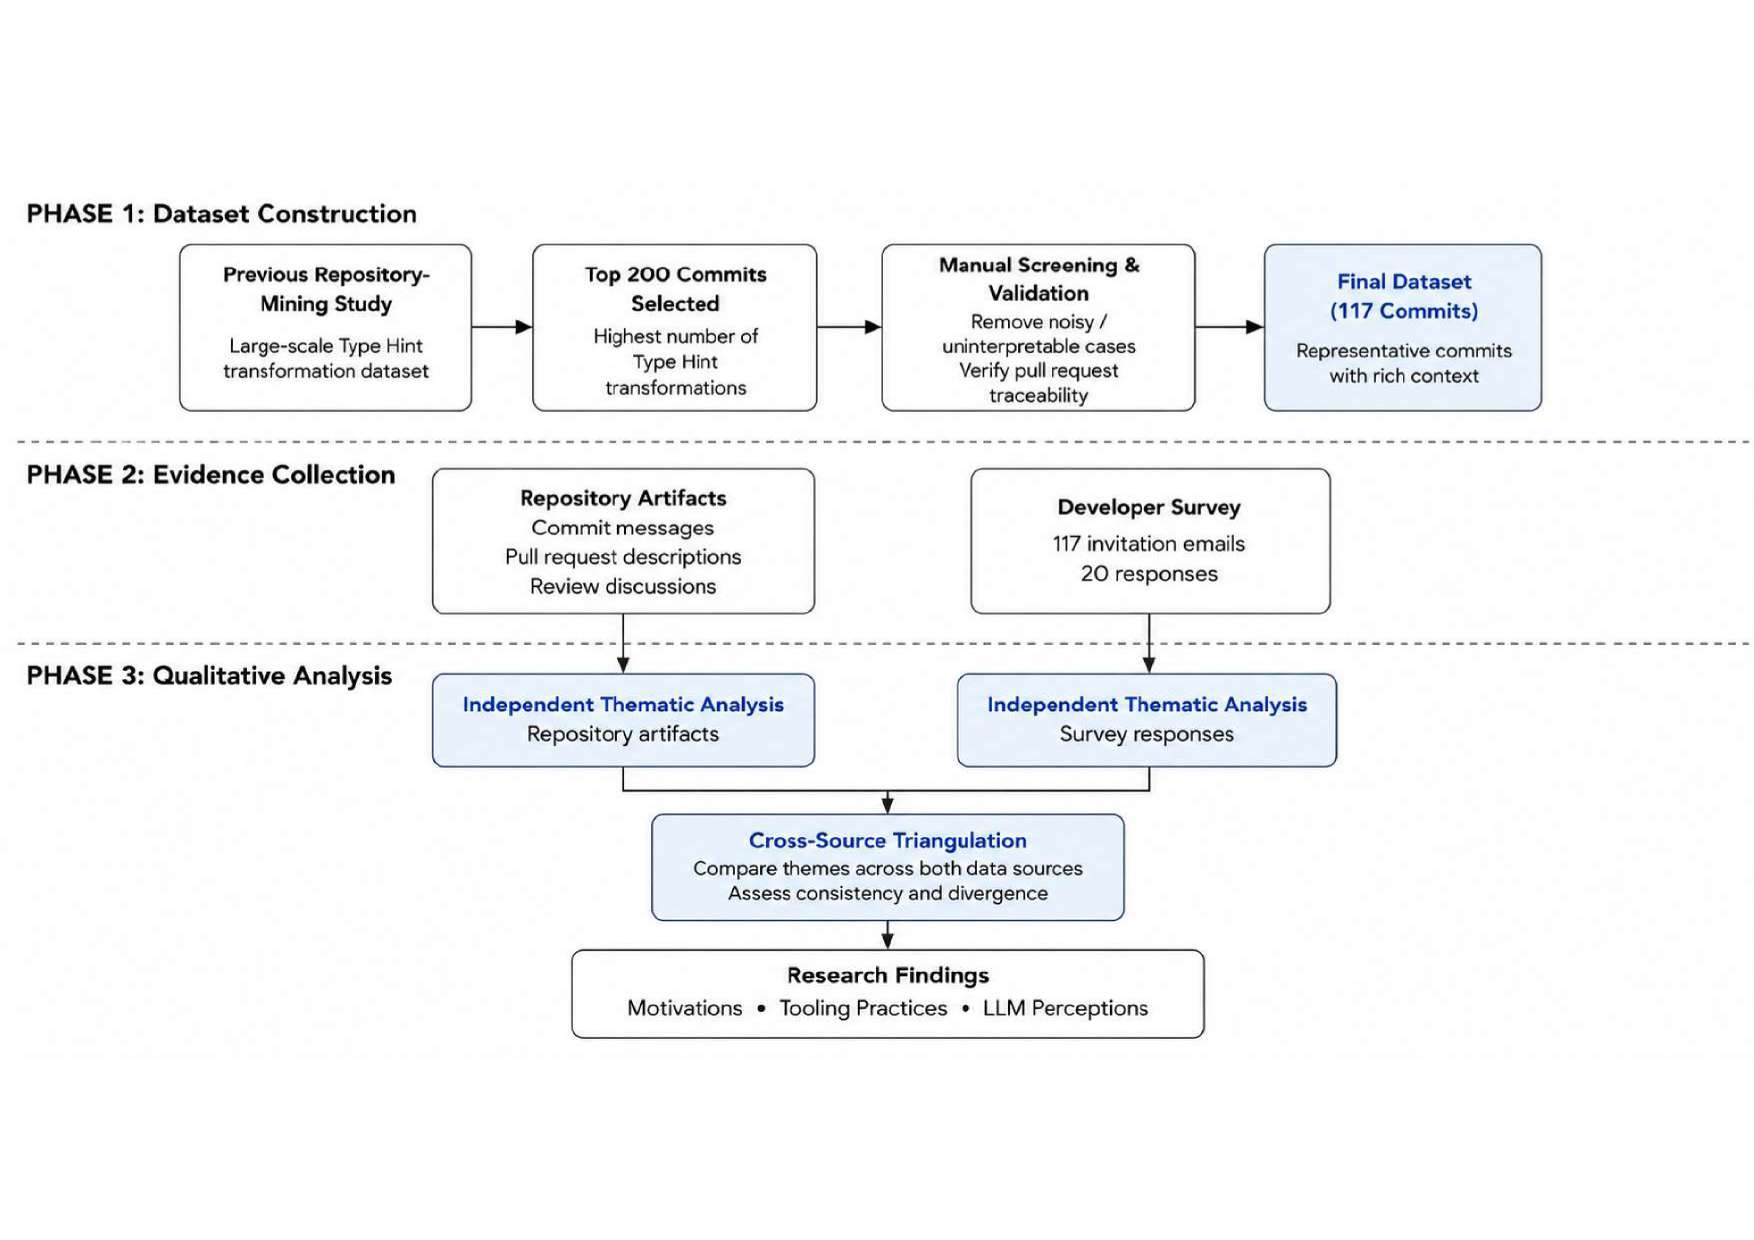
\includegraphics[width=\textwidth]{imgs/metodologia_horizontal.pdf}
    \caption{Overview of the research methodology.}
    \label{fig:methodology}
\end{figure*}

This study investigates the motivations and practices associated with large-scale Python modernization efforts involving \ths. Figure~\ref{fig:methodology} presents an overview of the research workflow. While our previous research (based on a large-scale repository-mining analysis) characterizes how these transformations occur, it does not reveal the reasoning behind developers' decisions, the role of automation in modernization, or developers' perspectives on emerging AI-based support. To address these aspects, we conducted a survey with authors of commits containing a large number of detected type-related transformations.

Specifically, we aim to understand why developers introduce and evolve type annotations, whether they rely on tools to support such modifications, and how they perceive the potential use of Foundation Models for similar tasks. To guide this investigation, we address the following research questions:

\begin{itemize}
\item \textbf{RQ1: What motivations drive developers to perform large-scale Type Hint modernization efforts?} This question investigates the related factors that motivate developers to modernize Type Hints across large open-source Python projects.

\item \textbf{RQ2: What tools or automation techniques do developers use to support large-scale Type Hint modifications?} This question investigates the tools, scripts, and automation strategies developers employ to facilitate large-scale Type Hint modernization.

\item \textbf{RQ3: How do developers perceive the potential use of Foundation Models to assist Type Hint modernization tasks?} This question seeks to identify developers' expectations, perceived benefits, concerns, and potential use cases for applying to Type Hint modernization.
\end{itemize}

We analyze survey responses using thematic analysis and integrate these findings with evidence extracted from commits and pull request discussions. We then perform a triangulation of evidence across the three sources (commits, pull requests, and survey responses), assessing consistency between observed code changes and developers’ reported motivations and practices.

This triangulation enables a more comprehensive understanding of large-scale \ths modernization by connecting observable software evolution with developer intent and decision-making processes.

\subsection{Study Settings}

We build upon a large-scale mining dataset of 141 popular Python repositories, selecting the top 200 commits with the highest number of \ths-related transformations. From this set, we manually curate a final dataset of 57 projects and 117 representative commits based on their relevance and the richness of contextual information available in the associated pull requests.

For each selected commit, we retrieve and analyze the corresponding pull request discussions when available. In cases where no pull request was explicitly linked, we manually verify the repository history to ensure traceability. Each commit is associated with a single primary pull request, and this relationship was validated manually.

To complement repository analysis, we contacted the authors of the 117 selected commits via email. Although 10 developers were unreachable, we obtained 20 valid responses from 20 different projects. The survey is exploratory in nature and aims to capture developers’ perspectives on motivations, tooling practices, and the potential use of Foundation Models in modernization tasks.

\subsection{Data Collection}

\subsubsection{Commit Selection}

Starting from the dataset produced in our previous study, we identified candidate commits according to two criteria: (i) the number of detected type-related source code transformations and (ii) recency, considering commits authored between 2024 and 2026. This subset accounts for 39.43\% of all detected transformations. To avoid over representing highly active contributors, we retained only the commit containing the largest number of detected transformations for each developer, ensuring that each developer was represented only once. These commits represent 24.28\% of transformations within the selected time period. We then excluded commits associated with GitHub \textit{noreply} accounts, since their authors could not be reliably contacted for the survey. The remaining commits were ranked according to their number of detected transformations then we selected the top 200, this subset covers 58.37\% of all transformations in the developers' largest commits during the selected period. Providing a manageable yet highly representative sample for the subsequent qualitative analysis.

\subsubsection{Survey Procedure}

We manually inspected each of the selected commits to assess whether the detected transformations were sufficiently evident and interpretable for a follow-up developer survey. Commits containing numerous unrelated modifications, where the detected transformations were part of broader code changes and their rationale could not be reliably inferred, were excluded. We also discarded cases lacking sufficient contextual information (e.g., commit messages or associated pull requests discussions) to support the qualitative analysis and survey design. This manual screening resulted in a final dataset of 117 commits.

We contacted the authors of the 117 selected commits through an e-mail survey containing the questions presented in Table~\ref{tab:survey_questions}. The questionnaire investigated (i) the motivations behind the transformations, (ii) the tools and automation practices adopted during the modernization process, and (iii) developers' perceptions regarding the use of language models for similar tasks.

\begin{table}[htb]
\caption{Script of the survey questions}
\label{tab:survey_questions}
\centering
\begin{tabular}{p{0.05\linewidth} p{0.80\linewidth}}
\toprule
\textbf{RQ} & \textbf{Question} \\
\midrule
RQ1 &
What was your decision-making process and rationale for introducing this change? \\

RQ2 &
Did you use any tools or automation to support this large-scale modification? \\

RQ3 &
Do you envision using language models to assist with this kind of task? \\
\bottomrule
\end{tabular}
\end{table}

Overall, we received 20 responses (17.09\% response rate), each from different open-source Python projects. The respondents include developers from widely used projects such as \textit{FastAPI}, \textit{aiohttp}, \textit{Scrapy}, \textit{MyPy}, \textit{Pipenv}, \textit{Locust} and \textit{Chia Blockchain}, including spanning domains. This diversity widens the range of perspectives captured.

\subsubsection{Repository Artifact Collection}

For each of the 20 survey responses, we collected the corresponding repository artifacts to support a triangulated analysis of software development decisions. Each case was anchored on a surveyed commit and expanded using the GitHub API to retrieve all associated contextual artifacts.

Specifically, we retrieved commit messages, pull request descriptions, and review-related discussions. Pull request data was obtained using the \texttt{/commits/{sha}/pulls} endpoint, while additional discussion context was collected using the issues and pull request review APIs, including issue comments (\texttt{/issues/{number}/comments}), review comments (\texttt{/pulls/{number}/comments}), and structured review events (\texttt{/pulls/{number}/reviews}). Consequently, each case in the dataset consists of multiple complementary sources of evidence: the developer's survey response, the associated commit message, the pull request description, and the corresponding review and discussion artifacts.

To construct each triangulated case, all artifacts were grouped by their associated commit and pull request identifiers, ensuring that all related discussion and review data were aggregated into a single analytical unit. This allowed us to capture both implementation-level decisions and the surrounding design rationale expressed during the review process.

To support qualitative analysis, the first two authors independently recorded observations for each case. For each artifact type, separate notes were produced summarizing the technical motivations, design considerations, and decision-making rationale expressed by developers across commits, pull requests, and review discussions.

\subsection{Data Analysis}
\label{subsec:data-analysis}

To investigate developers’ decision-making processes behind large-scale code changes, the use of tools and automation during these modifications, and their perceptions regarding the use of large language models (LLMs) to support such tasks, we analyzed 20 survey responses using thematic analysis following Braun and Clarke~\cite{Braun01012006}.

The unit of analysis consisted of two complementary data sources: (i) textual excerpts extracted from commits, pull request descriptions, and code review comments, and (ii) developers’ survey responses. Both sources were analyzed separately using thematic analysis. These excerpts were manually coded at a fine-grained level using a multi-label coding scheme, in which multiple codes could be assigned to the same segment when appropriate. The coding was performed explicitly, without inferring categories not directly supported by the text. Although most codes emerged from the data, some initial categories were informed by prior literature and were subsequently refined throughout the analysis process. Excerpts considered irrelevant according to predefined criteria—such as purely social interactions or comments without technical implications—were excluded from coding.

Following Braun and Clarke’s guidelines, the analysis proceeded through iterative cycles of data familiarization, code generation, grouping related codes into candidate themes, and continuous refinement until a stable thematic structure was achieved. Rather than following a strictly linear pipeline, the coding and theme refinement process was revisited multiple times to ensure consistency and conceptual coherence. The process was conducted in pairs, with independent coding by two researchers followed by comparison and reconciliation of differences. This cross-validation process helped increase consistency and reduce individual interpretation bias.

We also followed established practices for trustworthiness in qualitative research, including triangulation of interpretations between researchers, discussion meetings among researchers (peer debriefing), debate of individual perspectives during the analysis, investigator triangulation, and cross-checking of coding decisions until reaching consensus among the researchers~\cite{Nowell2017Trustworthiness}.

We used ATLAS.ti~\cite{atlas_ti} to support data organization, coding management, and traceability of analytical decisions, enabling an audit trail of code evolution and theme refinement. This contributed to the transparency and reliability of the analytical process.

Overall, the resulting themes characterizing developers’ motivations, modernization practices, and perceptions of AI-assisted transformations are presented in Section~\ref{sec:results}.


\subsection{Triangulation}

For each of the 20 cases, we performed a qualitative triangulation of developer intent by comparing the results of two thematic analyses: one conducted on repository artifacts (commit messages, pull request descriptions, and code review comments) and another conducted on survey responses. Each case corresponded to a single commit, its associated pull request and review discussion, and the corresponding developer survey response, treated as a unified unit of analysis.

The themes identified through thematic analysis were compared across these sources without re-coding the data, focusing on whether the same underlying motivation was expressed across different artifacts. This comparison assessed the degree of consistency between developers’ reported motivations and the motivations observed in repository artifacts.

Consistency was evaluated qualitatively based on the extent to which motivations converged across sources, considering both alignment and partial divergence in emphasis or detail.

This process was conducted independently by two researchers, and disagreements in interpretation were resolved through discussion until consensus was reached.

% % \todo[inline]{
% % TODO: reescrever o approach\\
% % - reasearch questions deve estar mais relacionadas as perguntas feitas aos devs\\
% % - explicar os parâmetros para coleta \\
% % - explicar como foi feito a analise temática\\
% % - referenciar commits que são exemplos de grandes refatorações em um único commit
% % }

% % \todo[inline, color = green]{Esse próximo parágrafo dá a entender que é só type-hints. Não vejo problema com isso, mas, se for desta forma, melhor revisar todo o texto para excluir structural pattern matching.}
% % \todo[inline, color=green]{E novamente, esse parágrafo também indica que a pesquisa se concentrou apenas em survey, mas outros pontos do texto fala em triagulação, análise de PRs, \ldots. Precisamos manter consistência no artigo.}

% \todo[inline]{adicionar iamgem da metodologia}
% % \begin{figure*}[t]
% % \centering
% % \includegraphics[width=\textwidth,height=0.35\textheight,keepaspectratio]{imgs/methodology.jpeg}
% % \caption{Overview of the research methodology, combining repository-based analysis, developer survey, and triangulation across multiple artifacts.}
% % \Description{A workflow diagram showing the research process. It starts with repository mining of Python projects, followed by ranking and selecting commits, manual curation to 117 commits, and branching into two paths: repository-based analysis (pull request analysis and commit-PR validation) and developer survey (data collection, responses, and thematic analysis). Both branches converge into a triangulation step that integrates commits, pull requests, and survey responses to assess consistency.}
% % \label{fig:methodology}
% % \end{figure*}

% This study investigates the motivations and practices associated with large-scale Python modernization efforts involving \ths. Figure~\ref{fig:methodology} presents an overview of the research workflow. While our previous research (based on a large-scale repository-mining analysis) characterizes how these transformations occur, it does not reveal the reasoning behind developers' decisions, the role of automation in modernization, or developers' perspectives on emerging AI-based support. To address these aspects, we conducted a survey with authors of commits containing a large number of detected type-related transformations.


% % \todo[inline, color=green]{Acho mais interessante o termo Foundation Models, em vez de large language models. Revisar em todo o artigo. Nem todo modelo de linguagem é de grande escala.}

% Specifically, we aim to understand why developers introduce and evolve type annotations, whether they rely on tools to support such modifications, and how they perceive the potential use of Foundation Models for similar tasks. To guide this investigation, we address the following research questions:

% \begin{itemize}
% \item \textbf{RQ1: What motivations drive developers to perform large-scale Type Hint modernization efforts?} This question investigates the related factors that motivate developers to modernize Type Hints across large open-source Python projects.

% \item \textbf{RQ2: What tools or automation techniques do developers use to support large-scale Type Hint modifications?} This question investigates the tools, scripts, and automation strategies developers employ to facilitate large-scale Type Hint modernization.

% \item \textbf{RQ3: How do developers perceive the potential use of Foundation Models to assist Type Hint modernization tasks?} This question seeks to identify developers' expectations, perceived benefits, concerns, and potential use cases for applying to Type Hint modernization.
% \end{itemize}

% Our study follows a mixed-method design. First, we build upon a large-scale mining dataset of Python repositories and select the top 200 commits with the highest number of \ths-related transformations. From this set, we manually curate a final dataset of 117 representative commits based on their relevance and the richness of contextual information available in associated pull requests.

% For each selected commit, we retrieve and analyze the corresponding pull request discussions when available. In cases where no pull request was explicitly linked, we manually verify repository history to ensure traceability. Each commit is associated with a single primary pull request, and this relationship was validated manually.

% To complement repository analysis, we contacted the authors of the 117 selected commits via email. Although 9 developers were unreachable, we obtained 20 valid responses. The survey is exploratory in nature and aims to capture developers’ perspectives on motivations, tooling practices, and the potential use of Foundation Models in modernization tasks.

% We analyze survey responses using thematic analysis and integrate these findings with evidence extracted from commits and pull request discussions. We then perform a triangulation of evidence across the three sources (commits, pull requests, and survey responses), assessing consistency between observed code changes and developers’ reported motivations and practices.

% This triangulation enables a more comprehensive understanding of large-scale \ths modernization by connecting observable software evolution with developer intent and decision-making processes.

% \subsection{Data Collection}
% \label{subsec:data-collection}

% % \todo[inline, color=green]{Importante reforçar não apenas os procedimentos do survey.}

% \subsubsection{Commit Selection}
% To complement the quantitative findings of our previous study, we collected qualitative evidence from multiple complementary sources, including repository artifacts (commits and pull requests) and a developer survey. Rather than relying solely on developers response, we combined the survey data with repository artifacts to enable triangulation between observed code changes and developers’ reported motivations and practices.

% Starting from the dataset produced in our previous study, we identified candidate commits according to two criteria: (i) the number of detected type-related source code transformations and (ii) recency, considering commits authored between 2024 and 2026. This subset accounts for 39.43\% of all detected transformations. To avoid over representing highly active contributors, we retained only the commit containing the largest number of detected transformations for each developer, ensuring that each developer was represented only once. These commits represent 24.28\% of transformations within the selected time period. We then excluded commits associated with GitHub \textit{noreply} accounts, since their authors could not be reliably contacted for the survey. The remaining commits were ranked according to their number of detected transformations then we selected the top 200, this subset covers 58.37\% of all transformations in the developers' largest commits during the selected period. Providing a manageable yet highly representative sample for the subsequent qualitative analysis.

% % For each selected commit, we retrieved and analyzed the corresponding pull request when available, ensuring traceability between implementation changes and their documented rationale. In cases where no pull request was explicitly linked, we manually inspected repository history to recover the most relevant contextual discussion.

% % Only after this full artifact-based filtering process did we contact developers via email to conduct the survey. After removing 9 unreachable contacts, we obtained 20 valid responses. These responses were then analyzed in conjunction with commit and pull request data as part of our triangulation strategy.

% % \todo[inline]{Tem que ajustar o parágrafo anterior com esse. Em alguns pontos, está dando a impressão que o survey é a fonte principal. Ela é super importante, mas as análises manuais de commits e PRs também são relevantes para a triangulação. }
% % \todo[inline]{Talvez incluir uma figura com cada passo para a construção do conjunto final. Iniciou com 200, aplicou um filtro que reduziu para ABC, outro filtro que, até chegar em 117 commits. Os parágrafos a seguir se concentram no survey. Seria legal enfatizat tudo.}

% % Next, we manually inspected the source-code changes and commit messages associated with each selected commit. The goal was to identify commits that best represented large-scale modernization efforts and provided sufficient context to answer our research questions. This curation process resulted in a final dataset of 117 commits.

% \subsubsection{Survey Procedure}
% We manually inspected each of the selected commits to assess whether the detected transformations were sufficiently evident and interpretable for a follow-up developer survey. Commits containing numerous unrelated modifications, where the detected transformations were part of broader code changes and their rationale could not be reliably inferred, were excluded. We also discarded cases lacking sufficient contextual information (e.g., commit messages or associated pull requests discussions) to support the qualitative analysis and survey design. This manual screening resulted in a final dataset of 117 commits.

% We contacted the authors of the 117 selected commits through an e-mail survey containing the questions presented in Table~\ref{tab:survey_questions}. The questionnaire investigated (i) the motivations behind the transformations, (ii) the tools and automation practices adopted during the modernization process, and (iii) developers' perceptions regarding the use of language models for similar tasks.

% \begin{table}[htb]
% \caption{Script of the survey questions}
% \label{tab:survey_questions}
% \centering
% \begin{tabular}{p{0.05\linewidth} p{0.80\linewidth}}
% \toprule
% \textbf{RQ} & \textbf{Question} \\
% \midrule
% RQ1 &
% What was your decision-making process and rationale for introducing this change? \\

% RQ2 &
% Did you use any tools or automation to support this large-scale modification? \\

% RQ3 &
% Do you envision using language models to assist with this kind of task? \\
% \bottomrule
% \end{tabular}
% \end{table}

% Overall, we received 20 responses (17.09\% response rate), each from different open-source Python projects. The respondents include developers from widely used projects such as \textit{FastAPI}, \textit{aiohttp}, \textit{Scrapy}, \textit{MyPy}, \textit{Pipenv}, \textit{Locust} and \textit{Chia Blockchain}, including spanning domains. This diversity widens the range of perspectives captured.

% \subsubsection{Repository Artifact Collection}

% For each of the 20 survey responses, we collected the corresponding repository artifacts to support a triangulated analysis of software development decisions. Each case was anchored on a surveyed commit and expanded using the GitHub API to retrieve all associated contextual artifacts.

% Specifically, we retrieved commit messages, pull request descriptions, and review-related discussions. Pull request data was obtained using the \texttt{/commits/\{sha\}/pulls} endpoint, while additional discussion context was collected using the issues and pull request review APIs, including issue comments (\texttt{/issues/\{number\}/comments}), review comments (\texttt{/pulls/\{number\}/comments}), and structured review events (\texttt{/pulls/\{number\}/reviews}). Consequently, each case in the dataset consists of multiple complementary sources of evidence: the developer's survey response, the associated commit message, the pull request description, and the corresponding review and discussion artifacts.

% To construct each triangulated case, all artifacts were grouped by their associated commit and pull request identifiers, ensuring that all related discussion and review data were aggregated into a single analytical unit. This allowed us to capture both implementation-level decisions and the surrounding design rationale expressed during the review process.

% To support qualitative analysis, the first two authors independently recorded observations for each case. For each artifact type, separate notes were produced summarizing the technical motivations, design considerations, and decision-making rationale expressed by developers across commits, pull requests, and review discussions.

% % We selected popular and actively maintained Python repositories hosted on GitHub using the SEART tool~\cite{Dabic2021}, following criteria inspired by previous mining studies~\cite{Zampetti2024}. The initial selection considered repositories that: (i) use Python as the primary language, (ii) are not forks, (iii) contain at least 1,000 commits, and (iv) have at least 10,000 stars. We additionally required recent maintenance activity within 90 days prior to data collection (April 2026).

% % We further refined the dataset by retaining only repositories with at least 10 branches, 30 contributors, and 100 forks. After manually removing tutorial-style and educational repositories, the final dataset comprised 141 projects.

% % We mined the complete commit history of each repository from January 2015 onward using our RefactoringMiner extension. The mining process was executed in batches to avoid memory limitations in large repositories and parallelized at the project level. After collection, the results were filtered to retain only transformations occurring in Python source files.

% % Overall, the resulting dataset contains more than 674,000 transformations across 127 repositories with at least one detected modernization instance.

% \subsection{Thematic Analysis}
% \label{subsec:thematic-analysis}
% % \todo[inline, color=green]{Citar o trabalho de Braun e Clarke. Essa seção não está muito bem escrita. O texto está todo na voz passiva, enquanto que o restante do artigo está na voz ativa. Parece uma lista de bullets. Acho que pode melhorar. }

% To investigate developers’ decision-making processes behind large-scale code changes, the use of tools and automation during these modifications, and their perceptions regarding the use of large language models (LLMs) to support such tasks, we analyzed 20 survey responses using thematic analysis following Braun and Clarke~\cite{Braun01012006}.

% The unit of analysis consisted of two complementary data sources: (i) textual excerpts extracted from commits, pull request descriptions, and code review comments, and (ii) developers’ survey responses. Both sources were analyzed separately using thematic analysis. These excerpts were manually coded at a fine-grained level using a multi-label coding scheme, in which multiple codes could be assigned to the same segment when appropriate. The coding was performed explicitly, without inferring categories not directly supported by the text. Although most codes emerged from the data, some initial categories were informed by prior literature and were subsequently refined throughout the analysis process. Excerpts considered irrelevant according to predefined criteria—such as purely social interactions or comments without technical implications—were excluded from coding.

% Following Braun and Clarke’s guidelines, the analysis proceeded through iterative cycles of data familiarization, code generation, grouping related codes into candidate themes, and continuous refinement until a stable thematic structure was achieved. Rather than following a strictly linear pipeline, the coding and theme refinement process was revisited multiple times to ensure consistency and conceptual coherence. The process was conducted in pairs, with independent coding by two researchers followed by comparison and reconciliation of differences. This cross-validation process helped increase consistency and reduce individual interpretation bias.

% We also followed established practices for trustworthiness in qualitative research, including triangulation of interpretations between researchers, discussion meetings among researchers (peer debriefing), debate of individual perspectives during the analysis, investigator triangulation, and cross-checking of coding decisions until reaching consensus among the researchers~\cite{Nowell2017Trustworthiness}. These practices contribute to the rigor and quality of the analysis, aligning with the concept of trustworthiness widely discussed in the qualitative research literature, particularly in terms of credibility, dependability, and confirmability, as proposed by Lincoln and Guba~\cite{guba1989fourth} and operationalized for thematic analysis by Nowell et al~\cite{Nowell2017Trustworthiness}.

% We used ATLAS.ti~\cite{atlas_ti} to support data organization, coding management, and traceability of analytical decisions, enabling an audit trail of code evolution and theme refinement. This contributed to the transparency and reliability of the analytical process.

% Overall, the resulting themes characterizing developers’ motivations, modernization practices, and perceptions of AI-assisted transformations are presented in Section~\ref{sec:results}.


% % We analyzed the collected transformations using exploratory data analysis and non-parametric statistical procedures due to the highly skewed nature of the data distributions. Our analysis includes temporal trends, commit-level transformation distributions, and authorship concentration metrics.

% % For temporal analyses, we used the Hamed--Rao modification of the Mann--Kendall test~\cite{hamed1998modified}. We also applied Mann--Whitney tests and Spearman correlation analyses when comparing groups and investigating contributor concentration patterns. Alongside statistical significance, we report effect-size measures for all analyses.

% \subsection{Triangulation}

% % \todo[inline, color=green]{Parte deste texto não estaria em data collection? Talvez seja essa parte que esteja faltando lá, para balancear melhor a importância do survey com outras coisas. Esse é um item mais crítico que eu gostaria que vocês revisassem.}

% For each of the 20 cases, we performed a qualitative triangulation of developer intent by comparing the results of two thematic analyses: one conducted on repository artifacts (commit messages, pull request descriptions, and code review comments) and another conducted on survey responses. Each case corresponded to a single commit, its associated pull request and review discussion, and the corresponding developer survey response, treated as a unified unit of analysis.

% The themes identified through thematic analysis were compared across these sources without re-coding the data, focusing on whether the same underlying motivation was expressed across different artifacts. This comparison assessed the degree of consistency between developers’ reported motivations and the motivations observed in repository artifacts.

% Consistency was evaluated qualitatively based on the extent to which motivations converged across sources, considering both alignment and partial divergence in emphasis or detail.

% This process was conducted independently by two researchers, and disagreements in interpretation were resolved through discussion until consensus was reached.
